% Source: 2006浙江文.pdf, source-relative PDF page 1, Q8.
% Visible vertices, midpoint labels, and edge visibility follow the printed diagram.
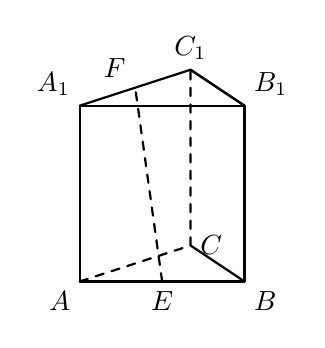
\begin{tikzpicture}[line cap=round,line join=round,x=0.95cm,y=0.95cm]
  \coordinate (A) at (0,0);
  \coordinate (B) at (2.2,0);
  \coordinate (C) at (1.48,0.48);
  \coordinate (Aone) at (0,2.35);
  \coordinate (Bone) at (2.2,2.35);
  \coordinate (Cone) at (1.48,2.83);
  \coordinate (E) at (1.1,0);
  \coordinate (F) at (0.74,2.59);
  \draw[thick] (A)--(B)--(Bone);
  \draw[thick] (A)--(Aone)--(Bone);
  \draw[thick] (Aone)--(Cone)--(Bone);
  \draw[thick] (B)--(C);
  \draw[thick] (Bone)--(Cone);
  \draw[thick,dashed] (A)--(C) (C)--(Cone) (E)--(F);
  \node[below left] at (A) {$A$};
  \node[below right] at (B) {$B$};
  \node[right] at (C) {$C$};
  \node[above left] at (Aone) {$A_1$};
  \node[above right] at (Bone) {$B_1$};
  \node[above] at (Cone) {$C_1$};
  \node[below] at (E) {$E$};
  \node[above left] at (F) {$F$};
\end{tikzpicture}
